\chapter{O InvestMVC}
Este capítulo evidencia como utilizar o software InvestMVC. O usuário pode logar no sistema, construir um robô de acordo com os parâmetros de entrada desejáveis e ativar o robô para que o mesmo opere de forma automatizada no Mercado de Moedas. Também é possível desativar o robô e consultar o histórico de operações (lucros ou prejuízos). Além disso, caso o usuário seja leigo no assunto de Mercado de Moedas, existe o FAQ com perguntas frequentes e conceitos chaves de mercado.

O código do software InvestMVC é aberto e pode ser clonado ou baixado no github\footnote{\url{https://https://github.com/cleitoncsg/investMVC/}}.

\section{Tela de boas vindas InvestMVC}

Ao acessar o software investMVC através do endereço do navegador localhost, irá aparecer a tela de boas vindas com animações. No canto superior direito, é possível logar no sistema (botão Entrar em cor verde) ou criar um novo usuário (botão Registrar em cor azul) conforme é evidenciado na Figura \ref{telaInicial}.

\begin{figure}[H]
\centering
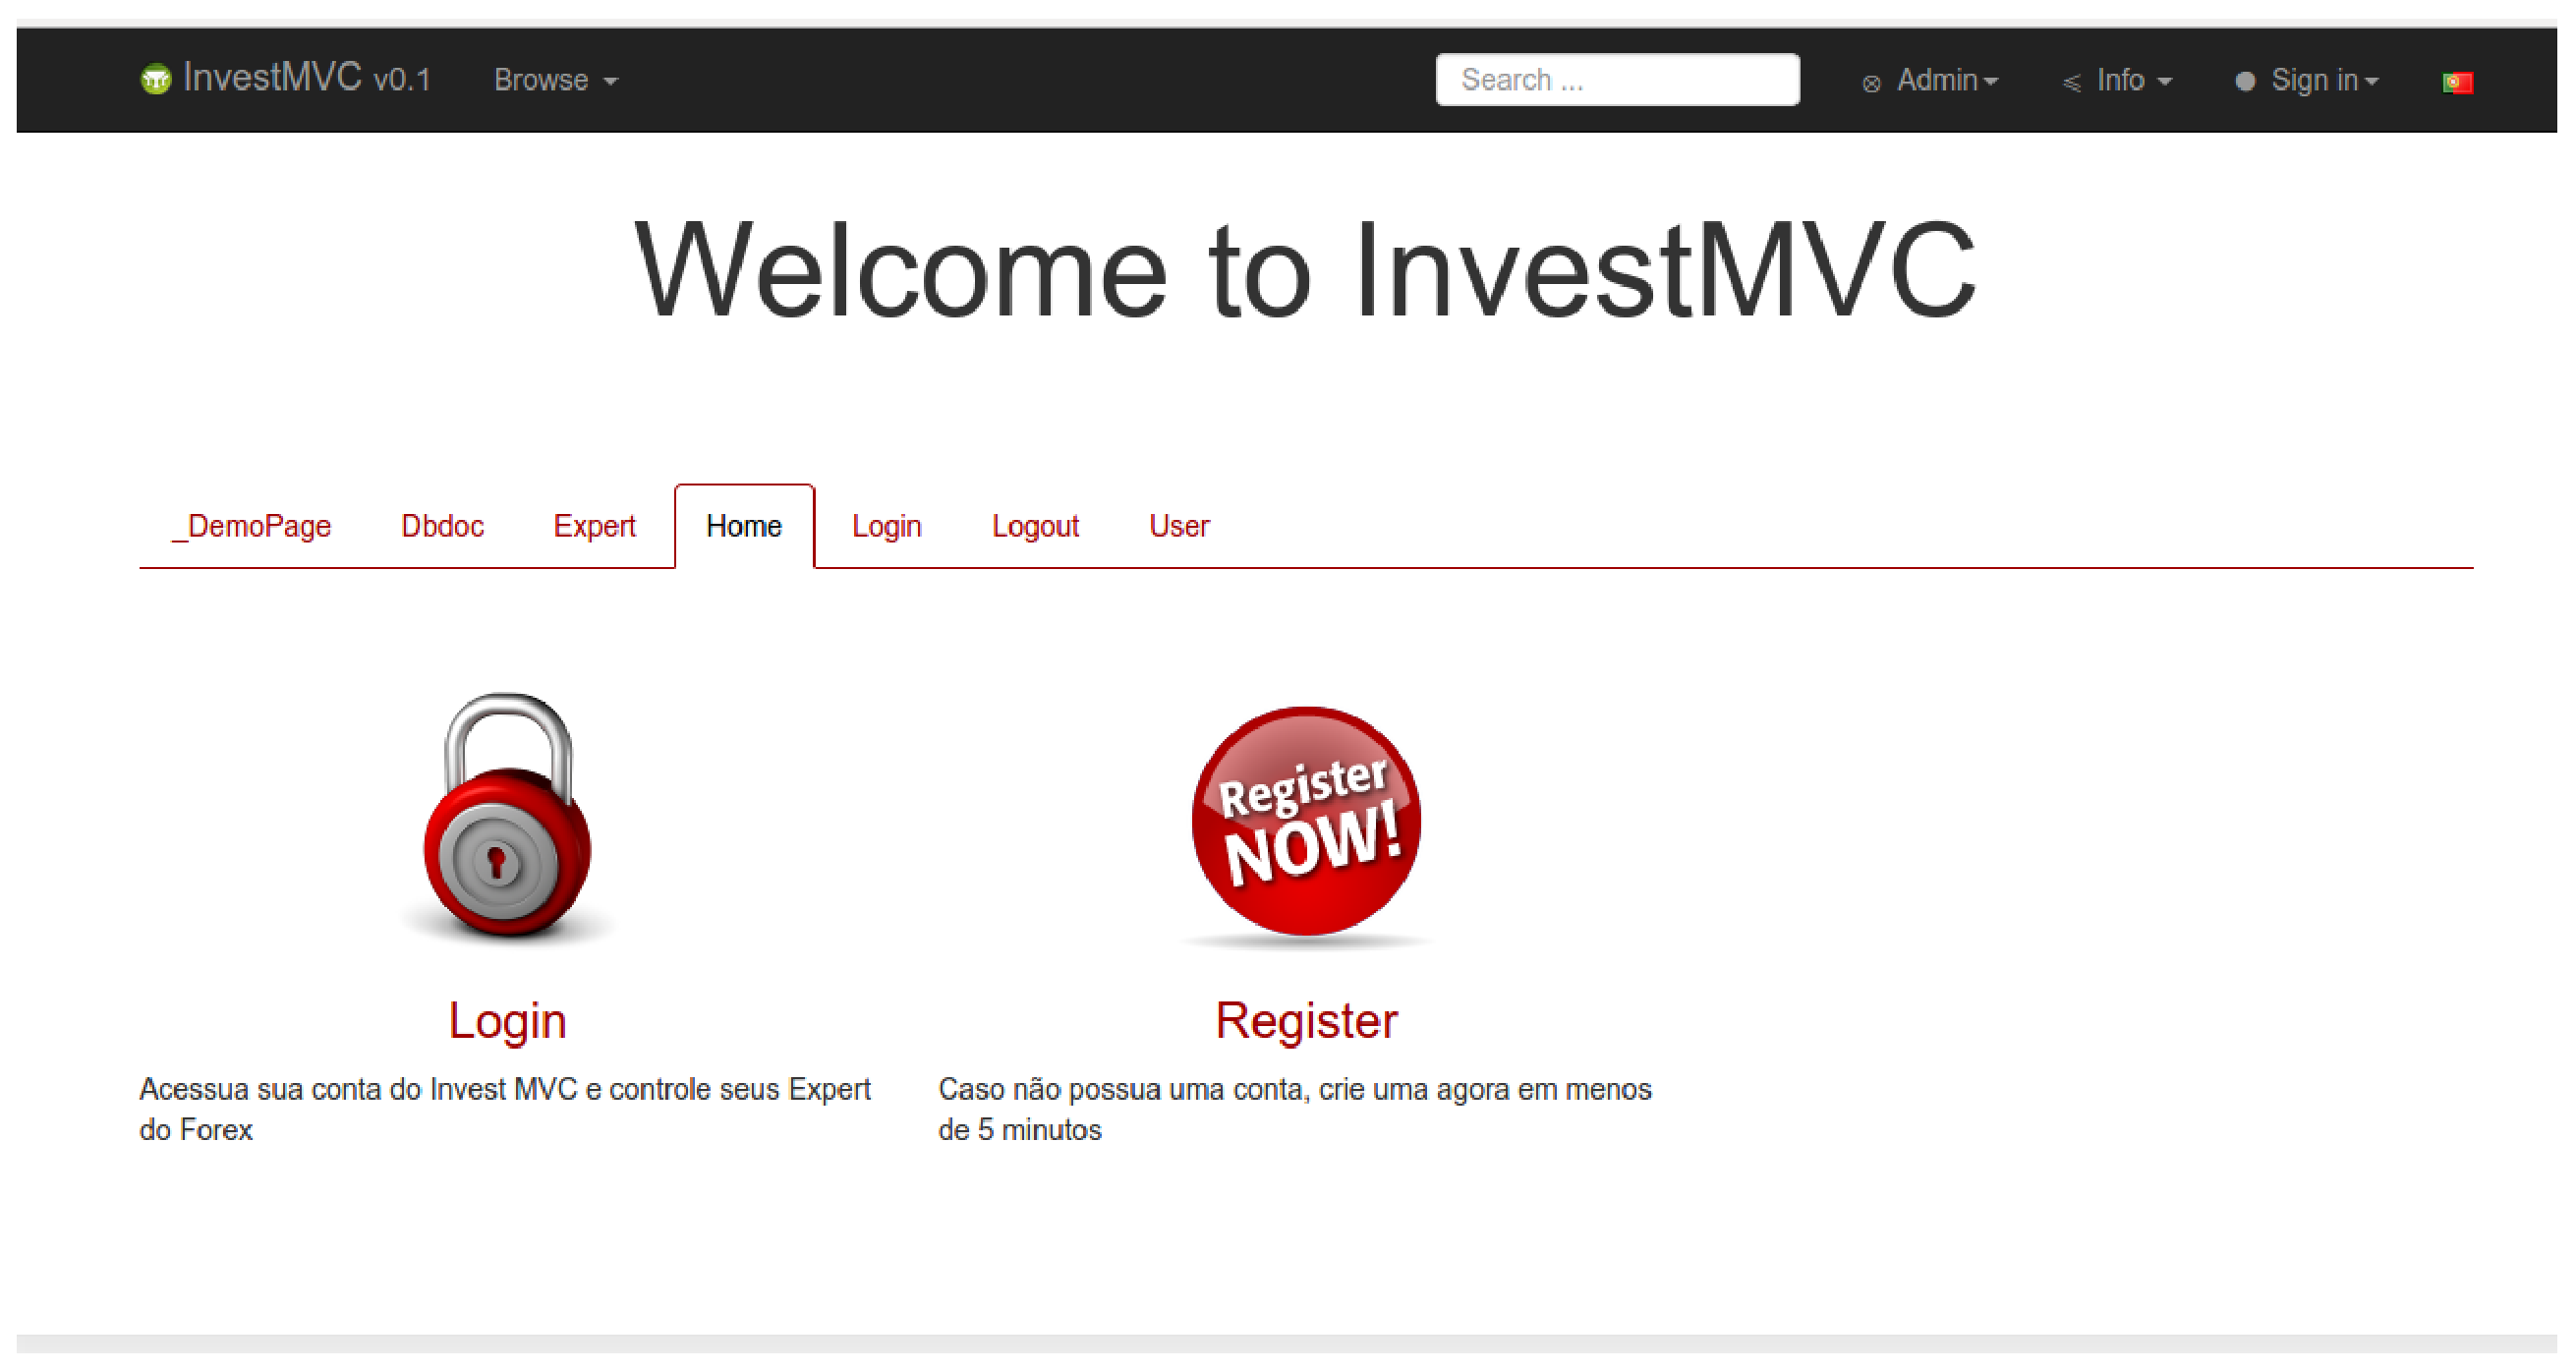
\includegraphics[width=0.9\textwidth]{figuras/telaInicial}
\caption{Tela de boas vindas InvestMVC}
\label{telaInicial}
\end{figure}

\section{Realizando o login}

Caso o usuário não tenha um login, basta criar um usuário com nome e senha conforme é evidenciado na Figura \ref{novoUser}. Após o usuário criado, basta fazer \textit{login} conforme é mostrado na Figura \ref{login}.

\begin{figure}[H]
\centering
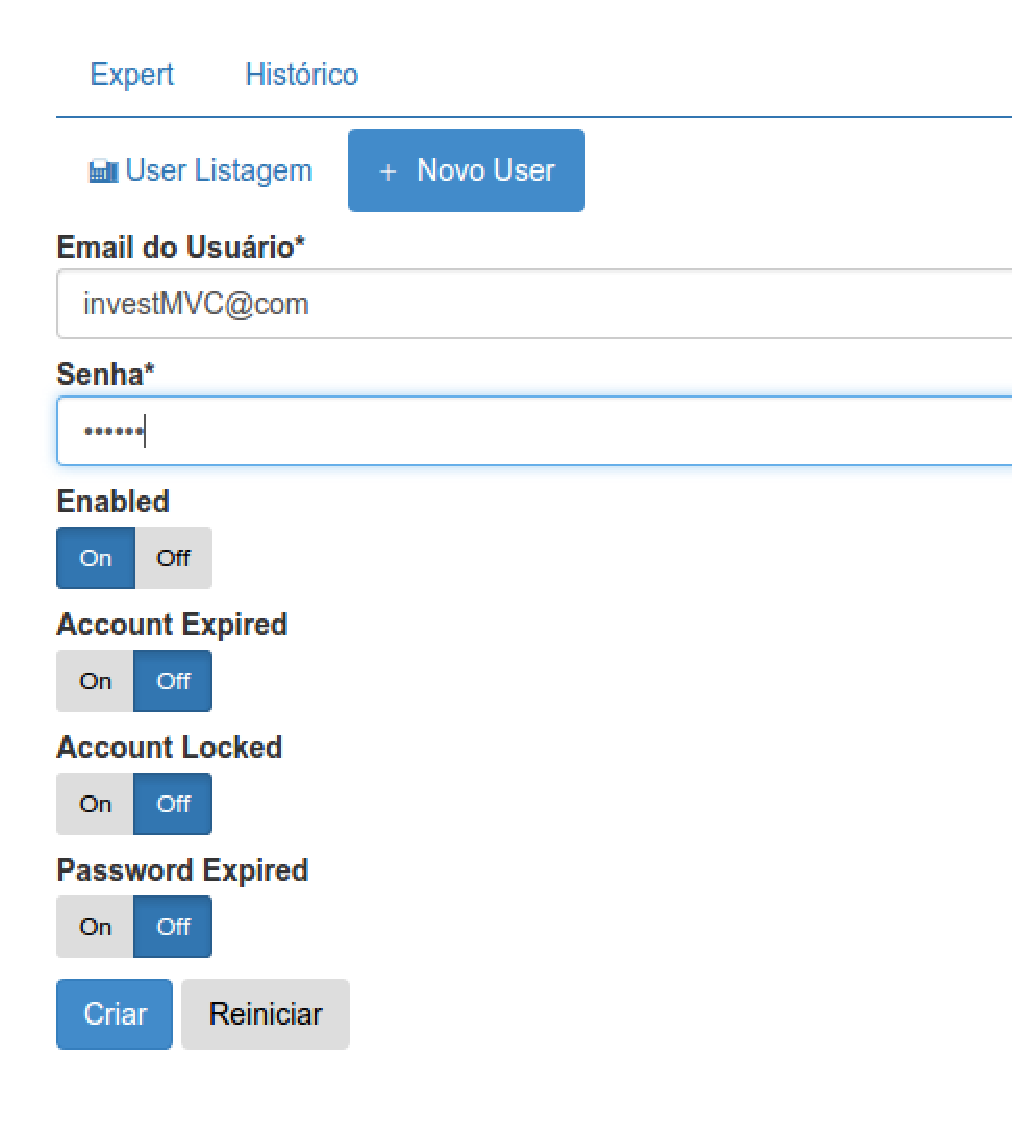
\includegraphics[width=0.9\textwidth]{figuras/novoUser}
\caption{Criando um usuário no software InvestMVC}
\label{novoUser}
\end{figure}

\begin{figure}[H]
\centering
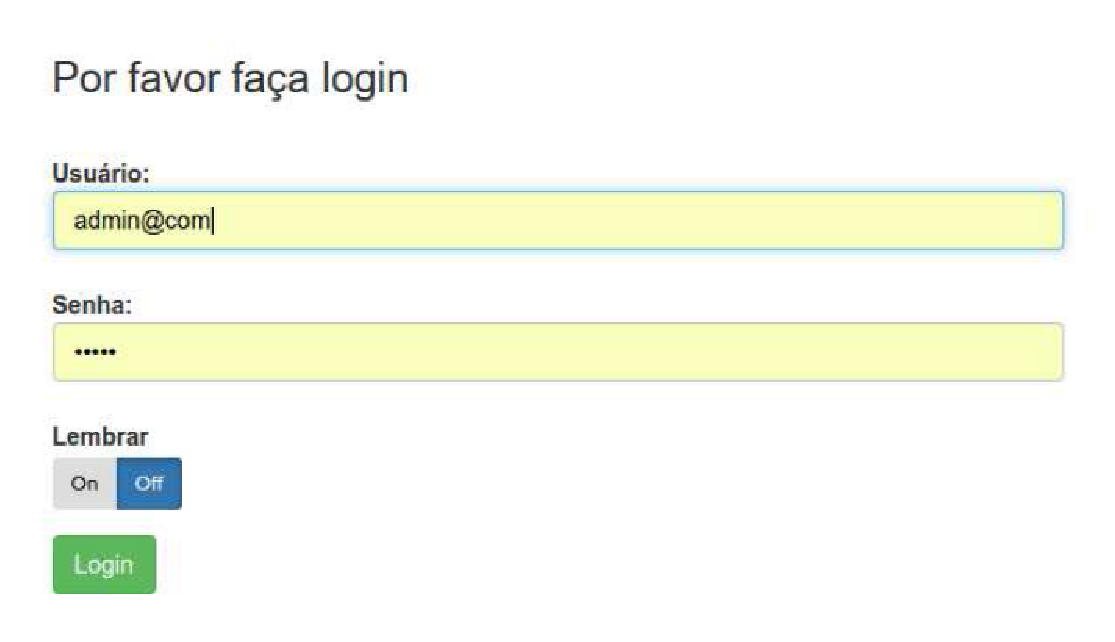
\includegraphics[width=0.9\textwidth]{figuras/login}
\caption{Tela de \textit{login} InvestMVC}
\label{login}
\end{figure}

\section{Suporte InvestMVC}
O software InvestMVC ajuda o usuário que tem pouco conhecimento sobre o Mercado de Moedas. Clicando no canto superior direito no botão “Suporte”, é aberta uma aba com os botões “FAQ” e “Conceitos” conforme é evidenciado na figura \ref{navSuporte}.

\begin{figure}[H]
\centering
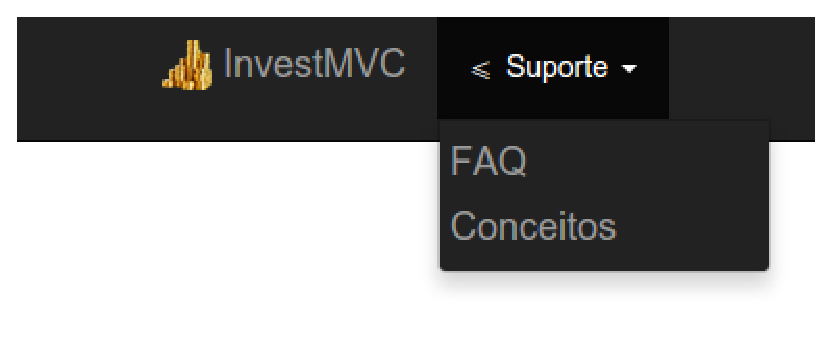
\includegraphics[width=0.9\textwidth]{figuras/navSuporte}
\caption{Suporte InvestMVC}
\label{navSuporte}
\end{figure}

Se o usuário selecionar a opção FAQ, é aberta a tela de “Perguntas Frequentes”, conforme é mostrado na Figura \ref{faq}. Essa tela ensina o que é o Mercado de Moedas, como funciona, como abrir uma conta para operar, quais são os riscos nas operações, entre demais informações. 

\begin{figure}[H]
\centering
\includegraphics[width=0.9\textwidth]{figuras/faq}
\caption{Tela de “Perguntas Frequentes”}
\label{faq}
\end{figure}

Para o usuário tem pouca noção de conceitos de mercado, como suporte e resistência, por exemplo, o software InvestMVC oferece a tela de “Conceitos básicos” com mais de 15 (quinze) conceitos, conforme consta na Figura \ref{conceitos}. 

\begin{figure}[H]
\centering
\includegraphics[width=0.9\textwidth]{figuras/conceitos}
\caption{Conceitos básicos de mercado}
\label{conceitos}
\end{figure}

\section{Criando um \textit{expert} no software InvestMVC}
É possível criar um \textit{expert} no software InvestMVC para operar de forma automatizada no Mercado de Moedas. Para isso, o usuário deve clicar no botão “Novo Expert” e selecionar o tipo de de gráfico (M5, por exemplo), o tipo de ordem (venda, por exemplo), os Métodos Matemáticos desejáveis para as operações de compra ou venda, o nome do \textit{expert} e quantidade de \textit{candles} (quantidade de gráfico de velas). Após preencher todos os parâmetros, basta clicar no botão “Criar”. Toda essa dinâmica de criação de um \textit{expert} é exibida na Figura \ref{criarExpert}.

\begin{figure}[H]
\centering
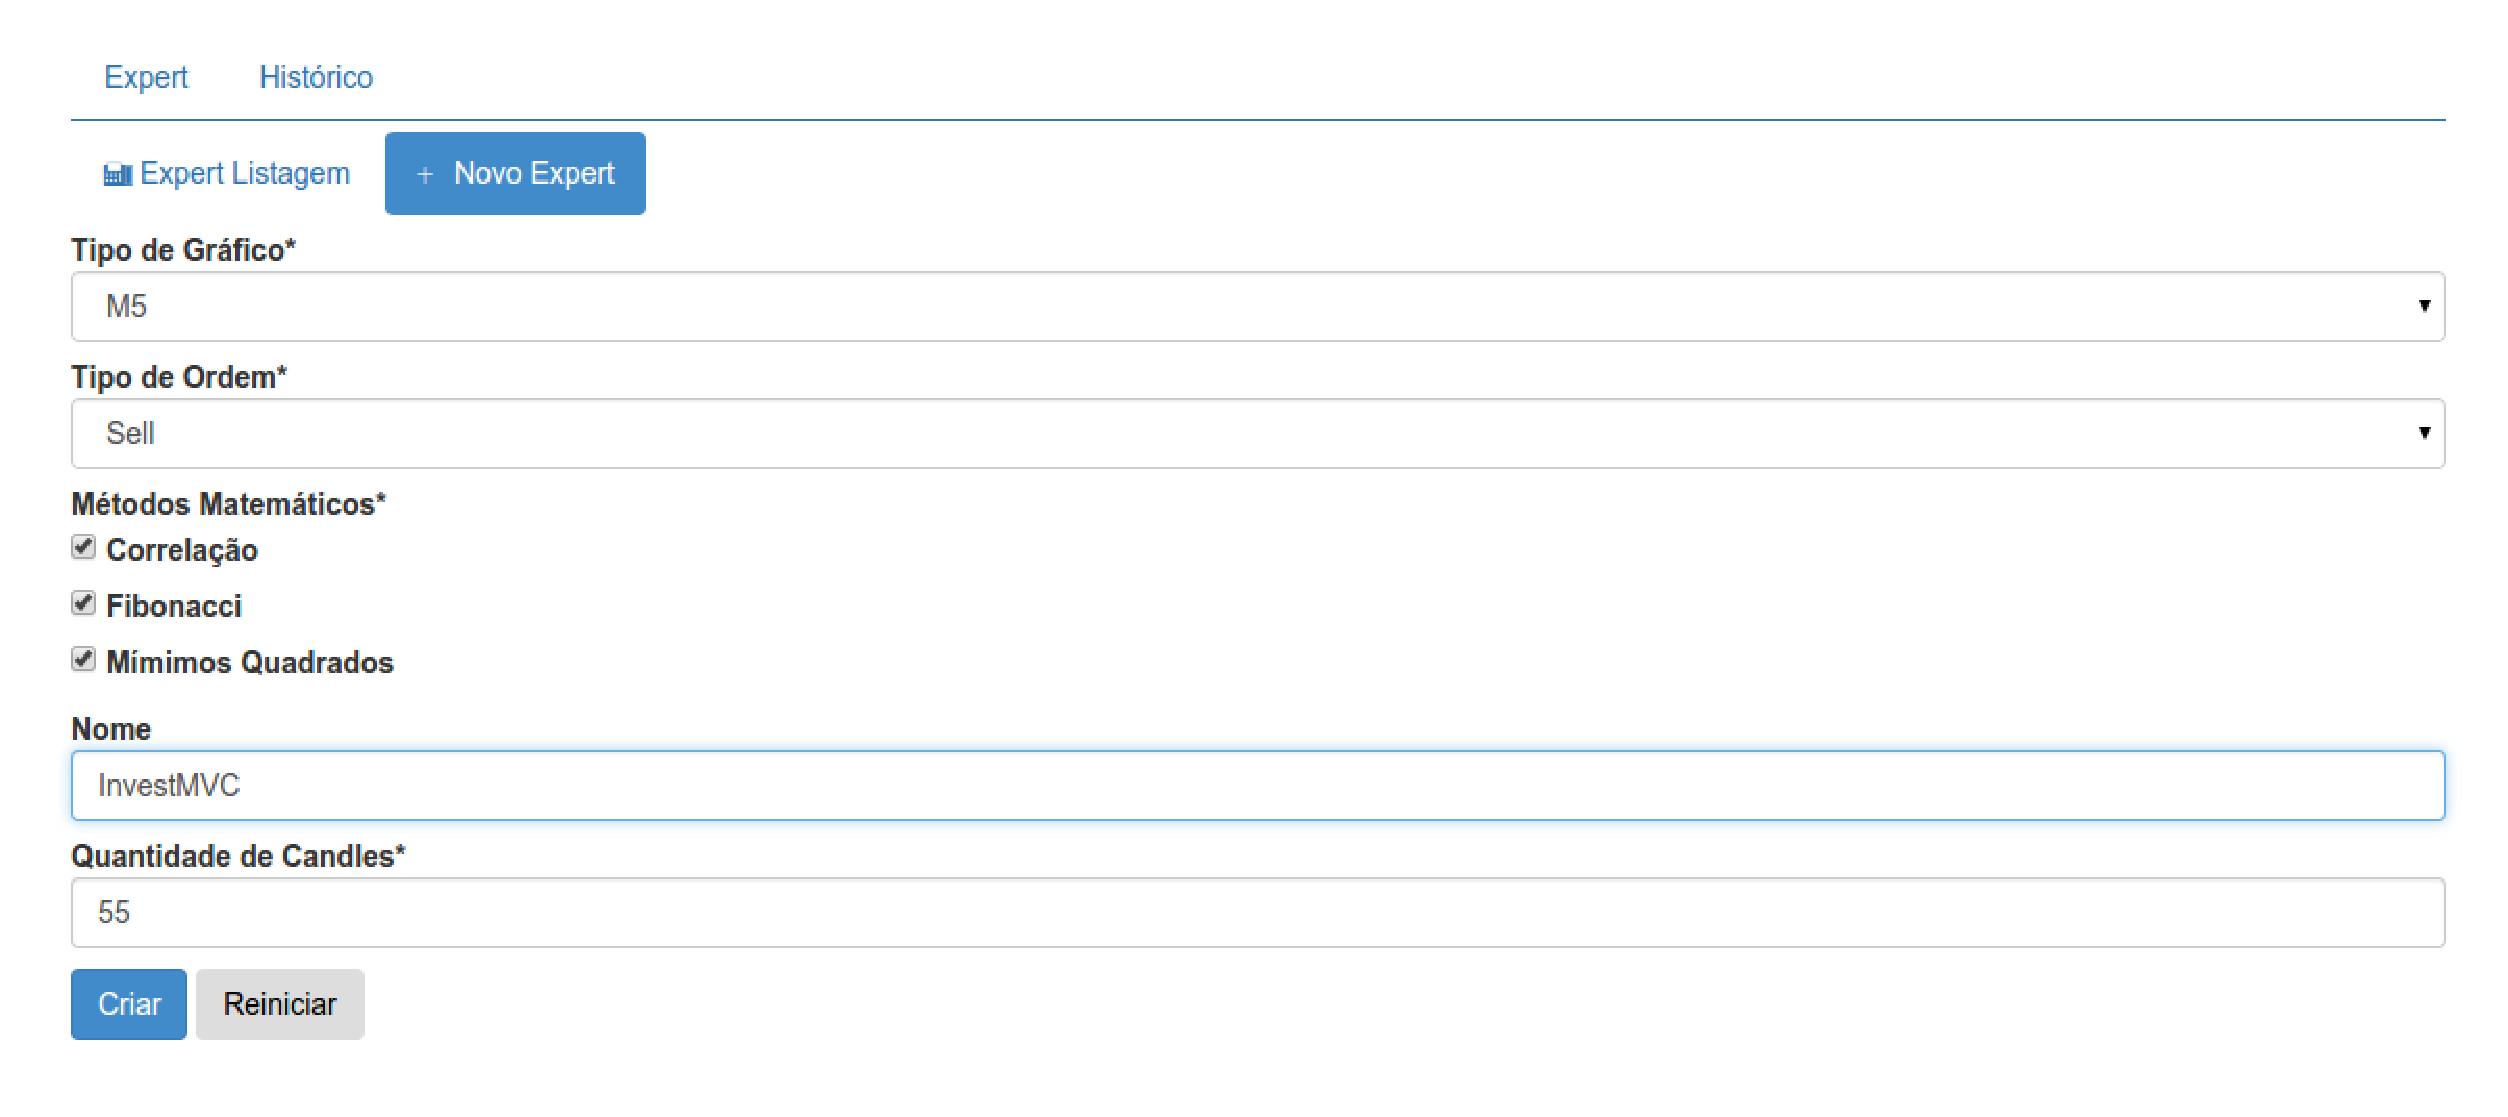
\includegraphics[width=0.9\textwidth]{figuras/criarExpert}
\caption{Criação de um \textit{expert}}
\label{criarExpert}
\end{figure}

Após criar um expert, o mesmo aparece na listagem de experts criados conforme consta na Figura \ref{ativado}.

\begin{figure}[H]
\centering
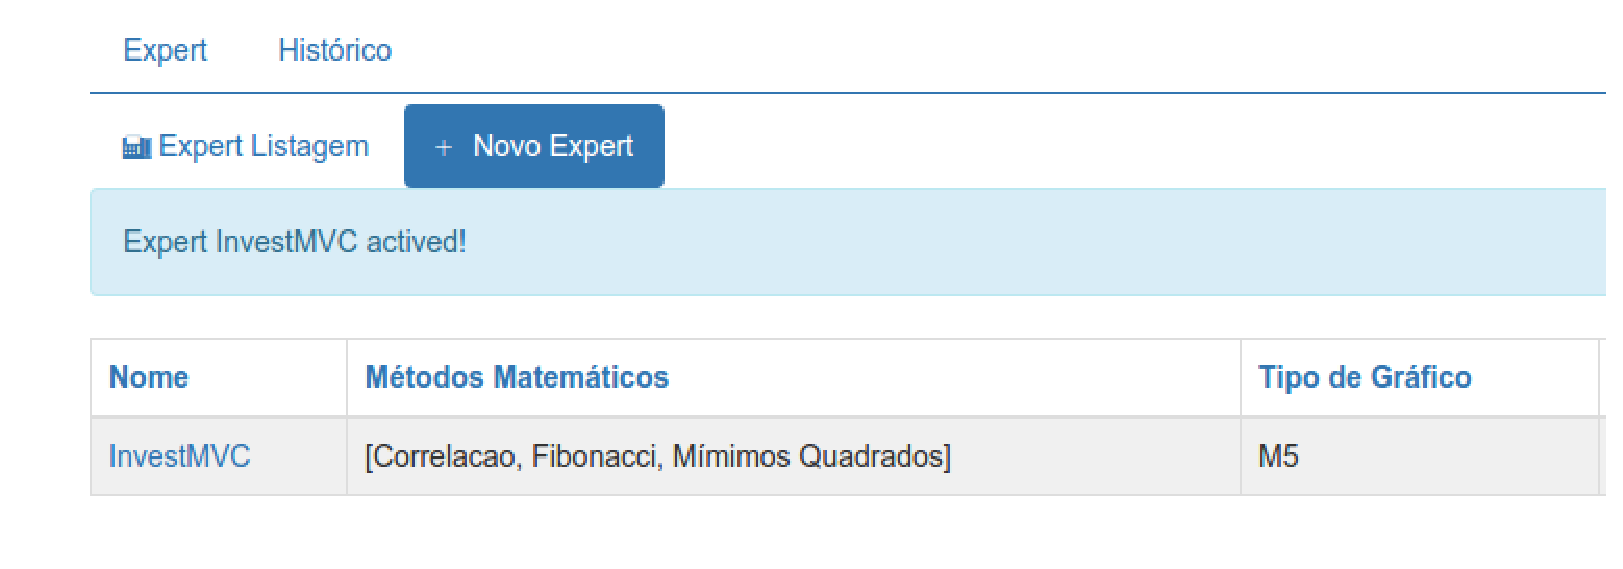
\includegraphics[width=0.9\textwidth]{figuras/ativado}
\caption{Listagem de \textit{experts} criados}
\label{ativado}
\end{figure}

Ao clicar no \textit{expert} da listagem é aberta uma tela mostrando todos os atributos pertencentes ao expert e o botão de “Ativar” (canto inferior esquerdo), conforme consta na Figura \ref{ativar}. Ao ativar o \textit{expert}, o mesmo já fica disponível para realizar operações de compra ou venda no Mercado de Moedas no par de moedas euro-dólar.

\begin{figure}[H]
\centering
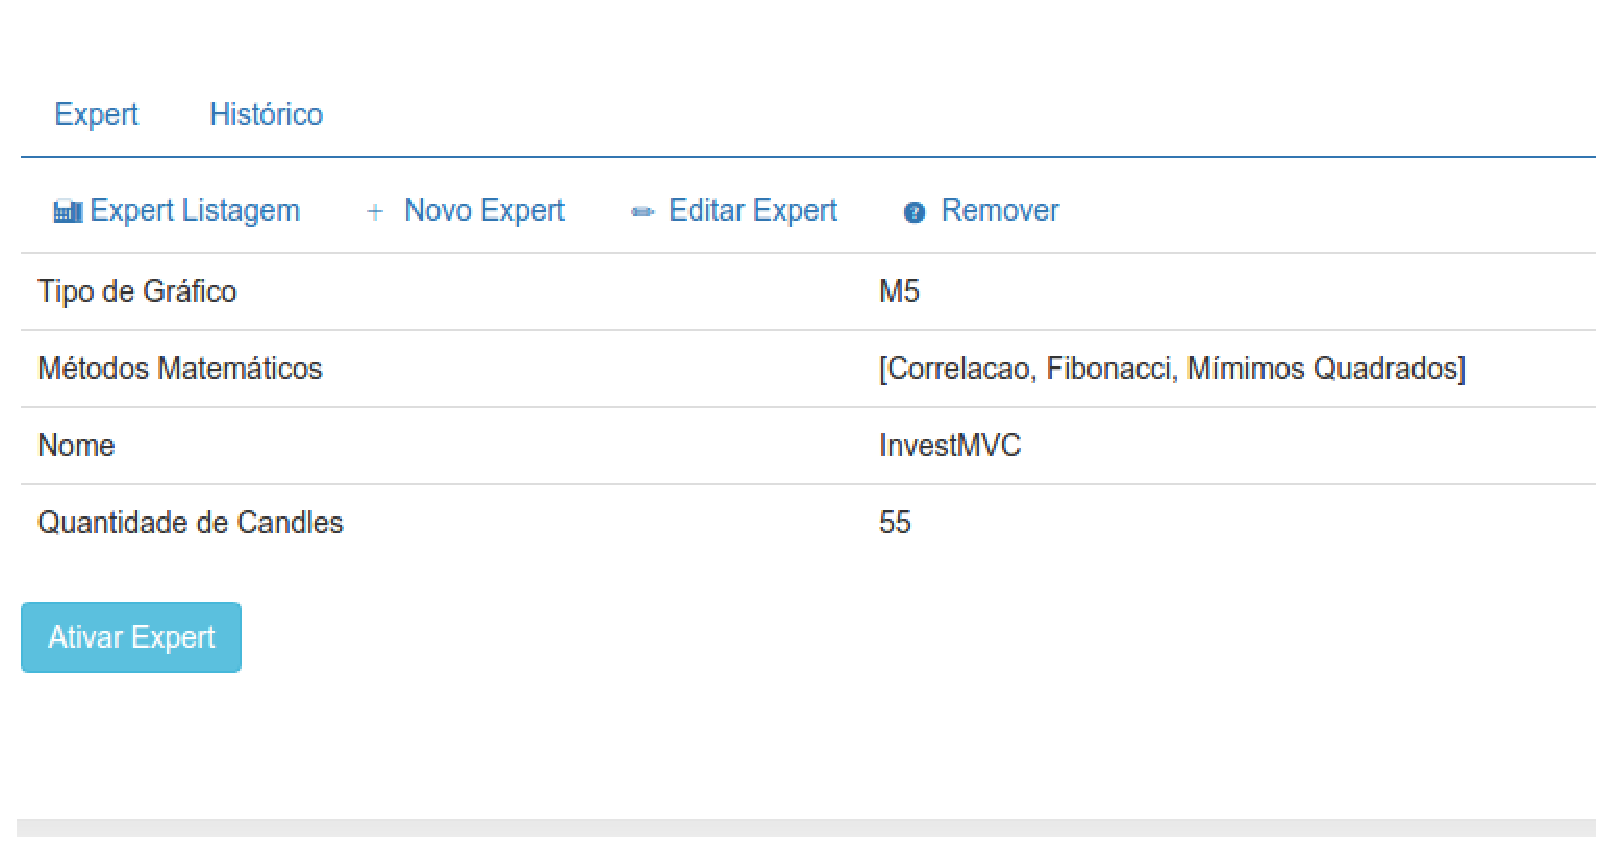
\includegraphics[width=0.9\textwidth]{figuras/ativar}
\caption{Tela de ativação de um \textit{expert}}
\label{ativar}
\end{figure}

\section{O software InvestMVC em ação}
Após criar um \textit{expert} e ativar o mesmo, é aberta a tela do MetaTrader mostrando os gráficos de operação e o \textit{expert} criado em ação. No retangulo em vermelho, é possível ver o \textit{expert} ativado fazendo os cálculos e esperando oportunidades para comprar ou vender no Mercado de Moedas conforme consta na Figura \ref{wine}.

\begin{figure}[H]
\centering
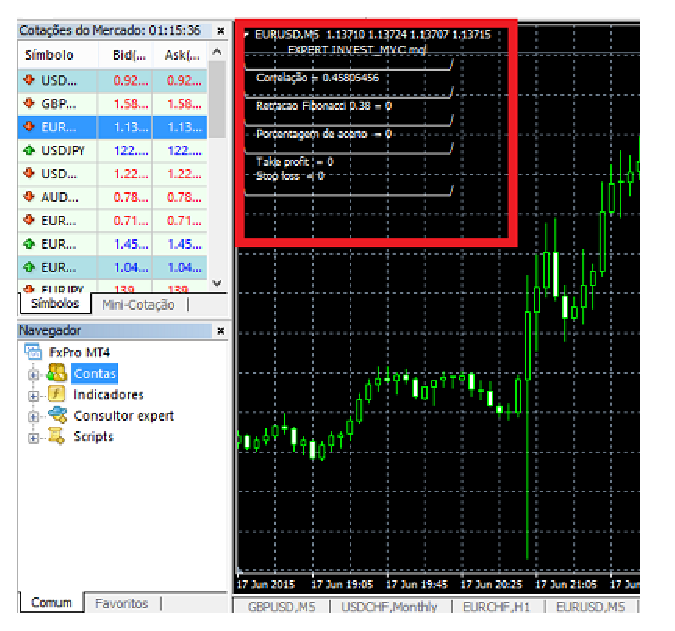
\includegraphics[width=0.9\textwidth]{figuras/wine}
\caption{Software InvestMVC em ação}
\label{wine}
\end{figure}
